\chapter{ 智能简史：生于数学，成于计算机}

 \begin{introduction}
  \item 从古代计数到现代计算的演进历程
  \item 数学思维在智能发展中的奠基作用
  \item 计算机科学的诞生与智能的机械化
  \item 关键历史人物与里程碑事件
  \item 从符号操作到机器学习的范式转变
\end{introduction}

“如果人们不相信数学很简单，那是因为他们没有意识到生活有多复杂。” 
\begin{flushright}
 ------约翰·冯·诺伊曼
\end{flushright}


智能的历史可以追溯到人类最早期的思维活动，而数学是其中最重要的基础工具之一。

对于古代人来说，数字的发明源于对数量的需求。无论是借助手指计数，还是用其他物体辅助，人类通过千年的发展，逐渐完善了从简单符号到抽象数字的演变过程。今天，我们的“自然数”概念似乎理所当然，但这一切都建立在人类历史上无数次的试错与进化中。


人类对“智能”的探讨源远流长。远在古希腊时期，哲学家们就已经开始追问：什么是智慧？什么是理性？我们如何通过思维去理解这个世界？从那时起，人们就梦想着创造能自主思考的机器。神话人物皮格马利 翁 (Pygmalion)、代达罗斯 (Daedalus) 和赫淮斯托斯 (Hephaestus) 可以被看作传说 中的发明家，而加拉蒂亚 (Galatea)、塔洛斯 (Talos) 和潘多拉 (Pandora) 则可以被 视为人造生命 (Ovid and Martin, 2004; Sparkes, 1996; Tandy, 1997)。

这些问题不仅关乎哲学，还对现代科学和技术的发展产生了深远影响。随着时间推移，这种对智能的追问从哲学的纯理论思辨，逐渐转向了科学与工程的实践领域。

早期的数学家如欧几里得、阿基米德以及笛卡尔等，通过逻辑和结构化的思维方式，奠定了后来发展计算机智能的理论基础。他们的工作不仅推动了科学与工程的发展，也为智能的理论构建提供了明确的框架。

\section{数字的起源，智能的开端}

%\section{计数工具的进化}
\subsection{手指：长在身上的计数器}
相信你在许多影视剧中都见过这样的一幕：一位算命先生，掐指一算，口中念念有词。这种“掐指一算”看似神秘，实则源自于古老而简便的计数方法。
\begin{figure}[htbp]
\centering
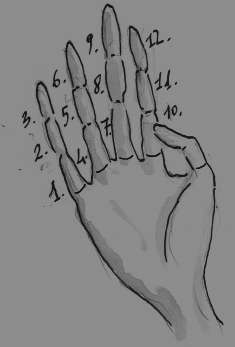
\includegraphics[width=0.5\textwidth]{figs/fingers.png} 
\caption{“掐指一算”}
%\label{}
\end{figure}

在远古时代，用双手的十根手指计数是再自然不过的选择。手指是人类最早的“随身计算器”，为我们提供了一个天然的计数系统，帮助我们轻松应对各种数量的计数、计算和记忆需求。通过简单的掰手指，人们可以记录日常生活中的数字，如牲畜的数量、物品的交换量，还可以推算季节、节气，安排农耕节日等重要活动。

%\subsection{手指计数与各种进制系统}
手指的构造与多种进制系统有着天然的联系。稍加思考，就可以发现十进制、二十进制、十二进制等计数法与手指构造的对应关系。

十进制(Decimal System)是最常见、最自然的计数方式。双手的十根手指自然与十进制对应，每根手指代表一个数字，从1数到10，完成一轮计数。十进制系统在全球的广泛使用，源于人类天生拥有十根手指的解剖学特征，正如爱德华·卢卡斯所言，这是为“自然界的一个偶然事件”​。

十二进制(Duodecimal System)则适用于更复杂的计数需求。除大拇指外的四根手指，每根手指有三段指节。一只手的大拇指指向四根手指的各段指节，可以计数1到12。一只手上计完12后，另一只手可以用来记录12的倍数。这种方式在古代美索不达米亚和古埃及文明中广泛应用，如今仍用于时间和角度的计数系统中，如12小时制、一年12个月以及节气的计算。

六十进制(Sexagesimal System)更为复杂，它通过结合双手来计数。一只手用于计12（与十二进制相同），另一只手的五根手指则记录12的倍数，因此五轮12等于60。这种计数方式适用于更大范围的计数。在古巴比伦时期，六十进制被发明并沿用至今，广泛用于时间和角度的测量系统，如1小时等于60分钟，1分钟等于60秒，以及360度的圆周划分。

二十进制(Vigesimal System)也是一种古老的计数法。在古代，一些民族为了更大范围的计算，除了用手指，还使用脚趾来进行计数。中美洲的玛雅文明和阿兹特克文明，以及现今的西非和欧洲部分地区，采用了以20为基数的计数法。

二十进制的痕迹在许多语言中依然存在。现代英语中的"score"一词（表示20）便保留了这一印记。例如，莎士比亚在《圣经》英译本中使用“three score and ten”（20的3倍加10，表示70岁)来指代古稀之年，而林肯在《葛底斯堡演讲》中使用“four score and seven years ago”(20的4倍加7，表示87)来表达87年前的历史。一百年后，马丁·路德·金在1963年著名的演说《I have a dream》中，也用到了这个词语，开头便是“Five score years ago”​（20的5倍，即100年前）​。如今，在现代英语中，“score”的这种用法已不再常见。

英国曾有一个结合十二进制和二十进制的货币系统。在这个系统中，1英镑等于20先令，1先令等于12便士。1971年，英国引入了十进制货币系统，1英镑等于100便士，先令在1990年后彻底退出流通。

在法语、丹麦语和巴斯克语中也能找到二十进制的痕迹。例如，法语中的数词从quatre-vingts（80）​、quatre-vingts-dix（90）​，到quatre-vingts-dix-neuf（99）​表明了凯尔特族过去采用的是二十进制计数法。同时，这些语言中还混杂了六十进制的痕迹，如数词soixante（60）到soixante-dix-neuf（79）​。

因此，手指不仅是我们身体的一部分，还是人类最早的天然计算工具。它帮助我们理解和组织世界，并为现代数学中的位值制和进制系统提供了最初的灵感。直到今天，手指仍是许多人在进行简单计算时的本能工具。可以说，手指是人类最早的“计算器”，引领我们从最原始的计数方法走向了复杂的数学世界。

\subsection{自然的教育：漂流孤岛，如何计数？}

假设你在一次航海探险中不幸遭遇风暴，被漂流到了一个无人孤岛。没有手表、手机，甚至没有任何现代工具，你如何计算时间？如何记录自己每天收集的食物？在这种完全回归自然的环境中，你必须依靠最原始的方式---刻痕与结绳计数法。

%当你孤身漂流到荒岛，没有现代工具，依靠刻痕或结绳来记录天数和食物数量，这种原始的计数方法正是人类最早期数字概念的萌芽。

虽然手指计数是人类最早的、天然的计数方式，但它的局限性在于只能处理简单的数值，且无法长久保存或传递信息。随着人类活动的日益复杂化，尤其是在贸易、农耕和时间推算时，需要一种能够长期记录和方便传递的计数方法。于是，结绳和刻痕等更抽象的计数方式应运而生。

通过在绳子上打结或在物体上刻痕，人类不仅可以记录更大范围的数字，还能保存和传递这些信息，这一进步标志着人类计数方法的进一步发展。

在一块石头或木头上刻下痕迹，记录每一天的过去，或者将一根绳子打上结，标记每天捕鱼或采摘的数量......通过这样的方式，你开始掌握数字的基本概念---记录、比较和计量。这是自然的教育，也是人类最早发明数字和计数系统的初衷，让生活更为便捷和高效。

\subsection{数字的诞生：从刻痕到符号}
正如在孤岛上刻痕记日，人类文明早期也经历了类似的阶段。人类的祖先首先通过在骨头、树木或石块上刻下记号，来记录天数、交易数量或物品的数量。这种刻痕计数法是最原始的记录方式，体现了数字发明的最早期形态。

随着时间的推移，单纯的刻痕已不足以满足日益复杂的需求。于是，人类逐渐发展出不同形式的数字系统。最著名的是古埃及的象形文字、古巴比伦的楔形文字，以及古代中国的结绳记事。每一个文明都在不同的环境下，发明了属于自己的数字记录方式，这些方式不仅记录数量，还用于交易、建筑和天文学等多个领域。

\subsection*{结绳计数：一种更高级的记录方法}
如果你在孤岛上拥有一根绳子，那么结绳计数法可能是比刻痕更便捷的方式。通过在绳子上打不同的结，记录每天的事件和物件的数量。这种方法历史悠久，曾被古代的中国和秘鲁等多个文明所使用。结绳计数不仅可以用于记载日常事务，还能帮助我们推测出早期文明如何进行复杂的交易和记账活动。

例如，古代秘鲁的印加文明使用一种称为“基普”（Quipu）的复杂结绳系统，记录农业产量、人口统计等信息。不同的绳子长度、颜色和结的形状代表着不同的信息。这种独特的系统不仅是数学记录的雏形，也是信息传递的早期方式。


随着人类文明的发展，人们逐渐认识到，仅依靠物理标记已不足以应对日益复杂的计算和记录需求，于是更加抽象的符号系统应运而生。在这一过程中，{\bf 阿拉伯数字}的发明中具有划时代的意义。相比于刻痕和其他早期符号系统，阿拉伯数字简洁易用，适合各种复杂计算，极大提升了计算效率，并最终成为全球通用的数字系统。  

与此同时，人们还逐渐发展出一系列数学概念和基本运算，如加、减、乘、除。这些数学工具不仅帮助人们更加有效地管理日常生活和建筑规划，还推动了贸易的发展，并促进了社会进步和技术革新。



\subsection{数字系统的进一步演化}
几千年来，人类都在探索如何建立数与物的对应关系，现代对数字的定义正是基于这种实践的延续。
刻痕和结绳只是人类早期计数和记录的开端。无论是结绳，还是在骨头、木棍上有序列地刻下划痕或是在容器中放置物品，这些方法已代表了相当抽象的符号系统，因为它们都与被计数的事物分离，既可以表示动物的数量，也可以记录借贷量或一个月的天数。一旦人类掌握了计数，数字系统的应用就变得“自然而然”了。或许正因如此，我们才称自然数为“自然”数(natural number)。然而，实际上，数字的概念一点也不“自然”。
%然而，距离现代数字概念的诞生，人类还需要跨越数百年的发展历程。

\subsection{数学与智能：从符号到计算}
数字的发明是人类探索数学的开端，也是数学发展的起点。通过数字，人类能够更高效地记录和处理信息，而这种能力为后来的智能模拟奠定了基础。事实上，现代计算机的核心正是基于数字的处理与计算。随着计算机的发明，智能的表达方式从早期简单的自然记录逐渐演变为依赖高度精确的数学运算和逻辑推理。

数学不仅为我们提供了表示数量的工具，还为理解和建模世界提供了逻辑框架，进而为智能的模拟和发展奠定了坚实的理论基础。
如同在孤岛上你需要依靠刻痕和结绳记录时间和数量，现代智能系统依赖数字符号和数学模型来执行计算和推理。数字不仅是简单的记录工具，更是推动现代智能技术发展的基础。
从几何推理到代数符号运算，再到概率论和统计学的建模，数学一直是理解智能和构建人工智能系统的核心。

%通过这个小故事引入，人类数字和计数系统的发明史与智能的发展历程紧密相连。从最早的刻痕和结绳记录，到符号系统的发明，再到现代计算机的数字处理，数学始终是智能发展的核心。


\subsection{数字的位值系统}
%\subsection{手写数字的位值}

在人类早期文明中，简单的手指计数和结绳、刻痕等计数方法已广泛用于记录数字，帮助人们应对日常的数值计算。然而，随着社会的发展和计算需求的提升，这些方法逐渐暴露出局限性，尤其是在处理更复杂和更大范围的数字时，显得低效而繁琐。 
为了解决这一问题，人类开始发明更加抽象和简便的符号系统来表示数字，从而催生了{\bf 位值制}这一革命性的数字表示方式, 使得复杂的数值能够通过简单的符号位置来表示和计算。

早期的计数系统大多采用{\bf 加法规则}。例如，在古代巴比伦的黏土板上，数字是通过符号的重复来表示的：数字“1”用一个符号表示，数字“2”用两个相同符号表示，数字“3”则用三个相同符号。
这种计数方式很眼熟，中文数字、罗马数字、古印度的婆罗门数字和笈多王朝使用的数字，以及大洋彼岸的玛雅数字，都采取了同样的方法。大多数的古代文明在表示前三个数字时，都采取了同样的方式：重复表示“1”的符号一次，两次，三次。古代的中文“一、二、三”、钟表盘上的罗马数字“Ⅰ、Ⅱ、Ⅲ”、阿拉伯数字也体现了同样的重复方式。可是，从数字4开始，所有的文明就都放弃了这种重复。为什么呢？

研究发现，人类的数感对少于3的数字有天然的反应，但超出这个范围后，单纯的重复符号便变得困难。对一些出生几个月的婴孩进行试验，结果证实人类与生俱来的数感的容量不超过三。

试想一下， 数字13若用重复排列“1”的符号13次来表示，无论是对书写还是阅读，都会很低效---怎么能一眼就看出它是13，而不是12或者14呢？

类似的问题在罗马数字系统中也很常见。罗马数字系统中，V表示5，X表示10，L表示50，C表示100。此外，向右添加符号为加，如，VI表示数字6，XI表示数字11；相反地，向左添加一个更小数值的符号为减，如IV表示4，IX表示9。
尽管使用了加减法规则的计数系统十分直观，但在表示大数时显得十分低效。例如1888年写成罗马数字就是MDCCCLXXXVIII，甚至无法有效表示类似100万那样的数字---除非把1000个M排成一排!

随着人类文明的发展，许多地区开始引入更为先进的计数法，其中最具革命性的是{\bf 位值制计数法}。古巴比伦、中国，尤其是印度和阿拉伯，率先采用了这种创新的位值制计数法。
这种计数法的关键在于符号的位置决定了其数值。例如，数字“12”和“21”虽然使用相同的符号，但因为符号位置不同，代表的数值也不同。

位值计数法具有出众的简洁性。%{\bf 阿拉伯数字}系统的简洁性更是让位值制达到了前所未有的高效性。
通过有限的符号，可以表达任意大的数值。
例如，$10^{100}$这个超出了物理限制的天文数字，在位值制下仅需101个符号即可表示---一个"1"后面跟着100个"0"。位值计数法用极短的符号链表示极其巨大的数值。

位值制不仅提高了数字的表示效率，还反映了数字的{\bf 对数增长}特性，即随着数字的增大，所需的符号长度呈对数增长，符号数量远远少于数字本身的大小。例如，表达$10^{100}$所需的符号长度约为$log_10 10^{100}=100$ (实际为101个)。
一般地，表达任意整数 $x$ 所需的符号数量接近 $log_{10} x$。
因此，从某种意义上，位值计数系统是最简洁、甚至最优的。

位值制的引入是人类计数方法的一次重大飞跃。从简单的重复符号到高度抽象的符号系统，位值制极大简化了计算过程，推动了计算和数学的发展， 奠定了现代数字系统的基础。
\section{ 位值制与对数增长在现代计算机中的应用}
在计算机科学中，在已经排好序的数组中查找某个元素的时间也是数组长度的对数。即使数组规模如同宇宙般庞大，经过几百次迭代后，便能够找到所需的元素---唯一的限制就是光速有限性所带来的信息传播和处理速度的物理极限。

%对数增长在现代计算机科学中扮演了关键角色，尤其体现在“地址”这一核心概念上。
%\subsection{URL与网络表示}
互联网的URL是位值制与对数增长在数据处理和网络寻址中的一个典型应用。 一个简短的URL(Uniform Resource Locator，URL，统一资源定位符)迅速定位到海量信息。
想象一下，你希望在网上搜索某项信息。尽管互联网上的数据量可能以EB($10^{18}$字节)甚至ZB($10^{21}$字节)计量，只要拥有对应信息的URL，你几乎瞬间就能找到目标信息。
这正是对数增长的强大之处：即使面对巨大规模的数据集，只需少量步骤就能完成检索。 

此外，URL的简短程度令人惊叹，其长度是整个网络大小的对数！这意味着我们可以轻松将URL存储在内存中，而URL指向的信息量却远远超出了其自身长度。
这种简洁有效的特性，展示了对数增长在计算与信息处理中的关键作用。

%\subsection{IPv4与IPv6的数据量级}
IPv4和IPv6的设计正是对数增长在实际应用中的另一个实例。
 IPv4地址使用{\bf 32位}二进制数来表示，每个IP地址可以被写成4个以点分隔的十进制数（如192.168.1.1），每部分对应一个8位的二进制数。
   32位的二进制能够生成$2^{32}$，即约{\bf 43亿}个唯一IP地址。这在IPv4设计之初被认为是足够庞大的数目。然而，随着互联网的迅速扩展，特别是物联网（IoT）设备和移动设备的广泛普及后，IPv4的43亿个地址空间将很快耗尽。

   为了解决这一问题，{\bf IPv6}应运而生。IPv6使用{\bf 128位}二进制数表示，由八组以冒号分隔的16进制数构成(如 2001:0db8:85a3:0000:0000:8a2e:0370:7334)。这种128位的二进制表示能生成$2^{128}$，即约{\bf $3.4 \times 10^{38} $} 个唯一IP地址，相当于为地球上的每粒沙子分配多个IP地址。这一数量级足以应对未来几十年甚至几百年内所有联网设备的需求。
   
%\subsection{对数增长与地址表示}
IPv4和IPv6的位数与它们能够支持的地址数量之间的巨大落差，展示了对数增长的强大力量。IPv4仅用32位符号就能表示43亿个地址，而IPv6仅用128位符号就能支持{\bf $3.4 \times 10^{38}$}个地址。随着位数的增加，IP地址系统实现了指数级的扩展，同时保持了地址表示的简洁性。

%再那些颠覆时代的宿命时刻中扮演重要角色的任务，如毕达哥拉斯，带有强烈的传奇色彩。他们埋头钻研不可能的问题，如化圆为方。他们将自己的才智倾注于探索数学的奥秘，创造了思维中的世界，并在其中找到了可以真实描述现代“宇宙工厂”的表达方式。不必借助幻想去解释这些宿命时刻的诞生，因为，正如茨威格所说，在那些超凡的时刻，“历史不需要帮助”。

会计师和土地测量师创造的技法构成了史前的算术和几何。那么，公元前5世纪的希腊到底发生了什么特别的事情，独独让这个时刻成为了数学史的开端呢?

公元前5世纪的重大革命，就是抽象的数学对象与自然中的实际物体之间的分离，即使数学对象本身就是从实际物体中抽象出来的也不例外。

自这场革命之后，数学研究的对象不再是必须与实际物体相关的几何图形和数字。研究对象性质的变化，最终引发了解决数学问题的方法的革命。让我们再来比较一下美索不达米亚泥板上的问题和毕达哥拉斯学派的问题各自的解决方法吧:第一个问题是通过计算解决的---做一个简单的除法就行了，而要解决第二个问题，就需要进行推理了。

在公元前5世纪的希腊发生的这场从计算到推理的转变，被视为数学的诞生。




纵观历史，数学的应用几乎渗透到了每一个领域中。
人类历史上的每一个重大事件的背后都有数学的身影：

-达芬奇的绘画（15-16世纪）

-哥白尼的日心说（16世纪）

-牛顿的万有引力定律（17世纪）

-马尔萨斯的人口论（18世纪）

-巴赫的12平均律（18世纪）

-孟德尔的遗传学（19世纪）

-晶体结构的确定（19世纪）

-人人平等（所有的直角都相等）、三权分立的政治结构（19世纪）

-无线电波的发现（19世纪）

巴贝奇的“机械”计算机（19世纪）

达尔文的进化论（19世纪）

爱因斯坦的相对论（20世纪初）

DNA双螺旋疑结的打开（20世纪）

冯.诺依曼的二进制编码和现代计算机（20世纪）

图灵机（20世纪）

……



\section{简明数学史}




让我们举一个经典的例子来说明这个问题。17 世纪时，继丹麦天文学 家第谷·布拉赫之后，约翰内斯·开普勒观察了行星围绕太阳的运动。他 意识到，行星的轨迹呈椭圆形。但椭圆的概念并不是为了描述行星的运 动才在 17 世纪发明出来的，人们早在公元前 4 世纪就已经知道什么是 椭圆了。为什么这个在古代诞生且与天体力学毫无关系的概念，却如此 适合描述行星的轨迹呢?换句话说，为什么行星会画出简单的几何图 形?或者回到刚才的问题，为什么行星的运动可以用数学表达式来描 述?面对这一惊人的事实，爱因斯坦总结道:“这个世界最不可理解之 处，就是它竟然可以被理解。”而尤金·维格纳则说:“数学在自然科学 中的巨大作用，没有任何合理的解释。” 

直到 16 世纪，人们仍然可以回答说“大自然根本不遵循数学规律”，然 后把这个问题扔到一边。这也是中世纪末期亚里士多德主义哲学的主要 观点。但从那以后，数学物理不断取得成功。人们不得不承认，就像伽 利略所说的那样，大自然这本大书是用数学语言写成的。 


“20世纪60年代，在量子力学的领域里流传着这样一句话：近些年来，物理学上“最重大的发现”是复数。那个时代的见证人之一尤里·马宁
[1]

就是这样认为的，他也是最早提出量子计算机想法的人之一。你们或许会问：复数怎么了？有什么重要的？如果你们以为复数的“复”是复杂的意思，而复数只是比你们常用的那些数字复杂一些，那你们的不以为意就可以理解了。马宁曾谈论过一些设想，而这些想法后来成为一个重要的物理理论的基础，他在那时讲述了这个故事。他认为物理学上的一些重要的东西具有某种数学形式，而在过去，这种数学形式与现实没有关联，当人们意识到这一点的时候，那个“疯狂”的想法就会实现。
一个关于数字的事件，你们尽可以想象这类数字有多复杂，它被列为物理学上的一个发现，甚至是“最重大的发现”，听到这里，你们或许会很[…]”


“在数字史中寻找隐藏着的“虚数的起源”时，我们会看到相当有趣的一幕：“一开始，人们在怀疑中排斥它，接着又在惊奇中重新认识它，看无法消除的它如何扰乱最敏锐的心灵。”韦达想把虚数从数学中彻底抹除，而笛卡儿在《几何》（1637年）中说：一个方程的根“不一定总是实数，有时只是虚构出来的数”。在邦贝利命名之后，笛卡儿也给那类数字取了名字，且这个名字沿用至今，即便---笛卡儿补充说---“有时候，根本不存在与那些虚构的数相对应的量”。
”

使用正确的表示法乃是兵家必争之地。这带领我们走到实际做研究的物理学家所熟知的另一个事实：研究物理时运用符号的有效性。
在最简单却深刻的层次上，代数是在某人引入文字代表数量的「想法」时诞生的。
不过更好的符号经常也表示对整个主题更深入的理解。在数学里也有基本上相当于寻求更完善符号的完整主题。


在1319年，奥卡姆这样写道:“Pluralitasnonestponendasinenecessitate.”意即“如无必要，勿增实体”。换句话说，简洁的理论更可取。
简洁是最大的精巧。莱昂纳多·达·芬奇(1452—1519)

追寻简单性的复杂旅程
你现在也明白了，奥卡姆剃刀是对抗过度拟合倾向的工具。奥卡姆剃刀提示我们，当每次发现新数据时，与其在相互竞争的各种理论之间来回切换，不如忽略那些过于复杂的理论，哪怕这会导致所有数据不能得到完美解释。毕竟，一般来说数据的成因众多，要进行完美的解释简直是天方夜谭。
骰子掷出6，空气中每个分子的位置都有可能对这个结果产生影响。然而跟踪空气中的每个分子并不现实，特别是因为这些分子的个数远远超出了时至今日制造的所有计算机的储存空间总和。
‘’第一个理解不进行完美解释的重要性的人大概就是被称为“现代科学之父”的伽利略。他最伟大的天才之举就是挑战亚里士多德的物理学，断言并不是越重的物体就天然地下落得越快。伽利略的这一思想又被称为自由落体定律，但它对于实验来说却是荒谬的。捡起一根羽毛和一块石头，然后让它们自由下落，你就会看到伽利略错了。
但伽利略的天才之处就在于，他理解到物体下落的内在性质只是它运动的一部分原因。各种物体都受到空气的作用力，而羽毛更甚。空气对较轻的物体的阻碍大于对较重的物体的阻碍，这种阻碍甚至可以让鸟类飞起来。伽利略因此提出，如果没有空气，那么空气的效应也会消失，而我们就会观察到物体本质的下落过程，它应该与物体的质量无关。伽利略指出，在真空中所有物体都会以相同的速度下落。

出于同一种思考方式，伽利略还有另一个天才想法，那就是相对性原理。这一原理断言，一个坐在船上没有窗户的密闭货舱中的人不可能知道这艘船是不是在运动。
不久之后，他对相对性原理的这种置信度让他将太阳放置在了宇宙的中心[7]。
在这两个例子中，伽利略的天才之处体现在他偏好原理的简洁与优雅，而非它们与实际的符合程度。这就是为了避免其他人陷进过度拟合的陷阱而应用奥卡姆剃刀的杰出例子。

半个世纪以后，轮到艾萨克·牛顿提出动力学基本原理，这一原理可以用4个符号来概括:。两个世纪后，詹姆斯·克拉克·麦克斯韦在说明他写出的方程可以同时解释电、磁和光的时候，强调的也是这些方程的简洁与优雅。所有这些绝妙的理论都基于同一个原则:去掉互不相容的多个特设解释，用简单而普适的原理来代替它们，哪怕要付出理论不能完美解释所有现象的代价。


世事并非一贯简单

然而，如果你相信最优秀的理论必定简单，那可就错了。气象模型的极端复杂已经众所周知，而现代神经科学强烈暗示，对人类大脑的理解不可避免需要复杂得可怕的模型---可能必须跟大脑本身一样复杂!
同样，2016年在围棋上打败李世石的人工智能AlphaGo也是如此复杂，必须用计算机才能将其表示出来。Cepheus和Libratus这两个在扑克上打败人类选手的人工智能也是如此[8]

实际上我们在讨论所罗门诺夫妖时，已经看到了研究某个现象所必需的复杂度是什么:数据(遵循的概率分布)的所罗门诺夫复杂度。即使艾伦·图灵当时没有认识到这个概念的形式定义，他对这个概念的理解却已经比任何人更深远。图灵于1950年发表的那篇具有历史意义的论文就已经提出了“能够跟人类一样说话的计算机最少需要多少复杂度”这个问题。依靠当时神经科学的初步进展，图灵估计，要建立能与人类一样进行交流的模型，最简单的算法也需要数十亿字节。也就是说，对于图灵来说，口头语中的所罗门诺夫复杂度大概就在十亿字节这个数量级上。我们会在第14章更详细地探讨这个话题。
同样，生物学、社会学与经济学中众多现象的所罗门诺夫复杂度可能远远超出这个数量，因此我们的大脑也就不可能理解这些现象，因为大脑储存空间的上限似乎只有几千万亿字节。因此，在面对生物学、社会学和经济学时，一切简单模型都必定失败。

交叉验证
在过度拟合与拟合不足之间找到平衡点是数据科学中的经典问题，通常被认为悬而未决。

拟合不足对应的情况是使用的学习算法过于刻板，无法很好地适应数据，因此导致预测中的偏差。要解决拟合不足的问题，最简单的办法通常就是增加学习算法的复杂度。一般来说我们可以增加参数的数目，然而，这样就会有过度拟合的风险。过度拟合就是过分贴近数据，因此训练集抽样中的随机因素对其影响过大。要避免这样的浮动，适当的做法是减少参数的数目。问题在于，要先验地得出合适的拟合程度是个棘手的问题，因为这似乎属于数据本身的内在性质。
在实践中，数据科学家会使用交叉验证的方法。对最优秀模型的搜索被分成两个阶段。首先，我们考虑那些复杂度不超过某个水平的模型，一般来说就是那些拥有至多个参数的模型，然后我们在其中选择能最好地解释训练集的模型。接下来我们会计算选出的模型在另一组被称为“测试集”的数据上表现如何。

所谓的交叉验证，就是优化这个复杂程度。首先从非常小的值开始，这时我们暂时处于拟合不足的区域中，考虑的那些模型过于死板，无法对数据进行解释。当增加时，算法在测试集上的表现会越来越好。这并不令人意外，因为我们允许模型拥有更大的灵活性。然而这种表现的上升在某一点处会停止，我们在这里就进入了过度拟合的区域。尽管最优秀的模型在训练集上的表现越来越好，但它在测试集上的表现自此之后却会降低。找到使这种转变发生的值正是对抗过度拟合这一危险的最好的方法之一(图12.1)。
%<!-- /var/folders/gl/1x3lhvs57l72x96lt82xqx_r0000gp/T/TemporaryItems/NSIRD_screencaptureui_tKxQcG/截屏2024-09-0320.33.23.png -->
图12.1实线表示训练集的错误率，模型的复杂度越大，这一错误率也越低。虚线表示测试集的错误率，它代表通过训练集计算而来的参数的泛化能力。我们看到在这里需要做出权衡。复杂度过高会损害泛化能力。

交叉验证中的值就是数据科学家所说的“超参数”(hyperparameter)。

蒂布斯兰尼正则化
让我们的大脑皮层以及其中大量神经元部分避免过度拟合的也许就是某种形式的正则化。毕竟，我们会活大约秒，但我们的大脑包含大约个神经连接，过度拟合的风险非常大。然而，正则化可以让我们根据抽样来调整模型的拟合程度。正则化技巧已经在实践中无数次证明了它们大有用处，这些技巧已经成为数据分析中不可或缺的工具，无论分析手段是线性回归、线性分类还是神经网络。

稳健优化
稳健优化的动机来自下面的观察:所有数据中都埋藏着不准确性甚至错误。在机器学习中，我们会说数据中有噪声。因此，所有通过优化得到的解答都必定只有在面对带有错误的数据时才是最优的。在面对正确的数据时，这些解答甚至可能完全不合适。
为了在数据存在噪声时仍然得到足够高效的解答，稳健优化首先会识别出一个不确定性集合6，其构造方式能使实际数据以非常高的概率处于这个不确定性集合之中。然后稳健优化会选择一个对于不确定性集合中的所有可能数据都有效的解答。更厉害的是，即使面对不确定性集合中最糟糕的数据，稳健优化也可以选择最合适的解答。它优化的是最坏的情况。
6在一维的情况下，不确定性集合对应的是置信区间。
令人惊讶的是，强调测量数据的不准确性可以让我们解释神经元经常不正常工作的有用之处。神经元欠缺稳定性实际上可能是一张王牌，而不是天生的缺陷。当某个神经元运行出错时，它会扰乱信号，就好像是有人为了在原始数据中加入不确定性而稍微改变了数据集那样。在一次又一次细化自身对于这个世界的模型后，我们的大脑会因此探索到各种不同的不确定性并为其做出调整，而不是配合只包含一开始那种噪声的数据。

更妙的是，无论是在不确定性集合还是在正则化中，所有看似随意的超参数实际上都证明了在寻找可信模型时先验置信度的不可避免性---或者说有效性!正则化很有用，因为它会迫使我们引入偏见。然而我们之前已经看到，偏见正是理性的支柱之一。
但纯粹贝叶斯主义者会在正则化与稳健优化的应用方法中看到欠缺之处。大部分机器学习算法最终会得出唯一一个模型，只会选择唯一一个理论。然而，集成学习或者自助投票等方法引导我们将不同的机器学习算法结合起来，尤其是可以利用Adaboost等技巧。这是因为，这些方法说明如果在优秀理论之间取平均值的话，通常得到的结果要比其中最优秀的理论还要好，因为这是对抗过度拟合的绝佳办法。互不相容的模型组成的森林要比其中每一棵树更睿智[15]。

许多研究人员已经意识到了这一点。例如在2016年，亚林·加尔发表了他的博士论文《深度学习中的不确定性》(“UncertaintyinDeepLearning”)，加尔在其中证明了机器学习中的大量常用技巧都可以用贝叶斯主义的语言重新诠释。我们刚才说到的随机失活正是这种情况!这是因为每一组失活神经元都对应着一个模型。因此，整个神经网络的预测可以通过取不同模型预测的平均值得到，其中每一个模型都可以由一组失活神经元得出。

只有贝叶斯推断才是可容许的※
甚至有一个定理强调了偏见的重要性:“没有免费午餐”定理。简单地说，这个定理断言不存在最好的机器学习算法。更准确地说，无论你用什么办法来选择模型，都存在这样的问题，你的方法会在这种问题上面被其他方法超越，而这些其他方法一般会利用适当的先验置信度。


但那是错的，不是吗?
请你也思考一下。在读到的时候，你有没有惊讶得跳起来?如果我跟你说勾股定理错了的话，你会有什么反应?如果我说，只是冒名顶替呢?引力并不存在呢?地表在向上加速移动呢?与通过杂交得到的品种相比，通过CRISPR基因编辑技术得到的转基因作物无论对人体还是对生物多样性来说都更有益呢?物理学家达成了光子(量子状态)的瞬间转移呢?存在并非有限也并非无限的集合呢?
否定那些违反直觉的奇怪假说不算是个坏习惯---虽说仅仅因为碰到这种假说就一脸敌意也不可取。如果我跟你说，我轻轻松松就登上了喜马拉雅山脉上的一座高峰，即使你不相信我，我也不会责怪你。在前几章里，我甚至还在为偏见辩护。不要浪费太多时间去仔细思考那些我们完全有理由认为没什么前途的想法。
同样，过去的智者与大型团体为了让自己看起来更可信，会激烈反对那些他们觉得过于违反直觉的想法。传说毕达哥拉斯学派淹死了可怜的希帕索斯，因为他证明了是个无理数;1632年，耶稣会2禁止数学中的无穷小计算[4];19世纪末，格奥尔格·康托尔提出的无限集合引来了同时代人的嗤笑，尤其是来自利奥波德·克罗内克的猛烈批评，他用到了类似“招摇撞骗”“叛徒”和“腐蚀青年人”等侮辱性的字眼;即使到了20世纪70年代，曼德尔布罗分形那种不同寻常、粗糙不平的新几何结构也被同时代的许多著名数学家激烈攻讦，对他们来说，真正的几何结构应该是平滑、连续、可微分的[5]。然而，在所有这些例子当中，数学界并没有把对新想法的否定一直持续下去，而是一步一步最终改变了想法，从过去的怒火中烧变成了今天的焚香供奉。今天，的无理性、莱布尼茨的微积分、康托尔的无限集合以及曼德尔布罗的分形都被视为数学中的珍宝。即使是这个等式，最终也有顶尖数学家为其辩护，比如斯里尼瓦萨·拉马努金、戈弗雷·哈罗德·哈代和陶哲轩[6]。人们有时候会说，数学这门科学能够扫清疑问、分辨真假，那么其中怎么可能发生这样的思想转变呢?数学家是怎么知道自己错了的?又是什么让他们回心转意?

2耶稣会是天主教会的著名修会之一，以保守而著称。---译者注
“新的科学真理最终取得胜利，靠的不是说服反对者并让他们理解，而是因为这些反对者最后都死了，而熟悉这个真理的新一代成长了起来。”物理学家马克斯·普朗克曾这样断言。根据数十年的心理学实验结果，心理学家多米尼克·约翰逊和詹姆斯·福勒这样补充道:“人类有着众多的认知偏差，但其中最常见、最严重也最普遍的就是自信过度。”科学家也无法免于这种自信过度。
往往只有少数人会花精力去理解其他人得出某个结论的理由，而更少见的就是那些尝试思考自己为什么会做出某种思考的人。而这本书的主要目的之一，正是引导你仔细思考是什么原因使你做出了某种思考!我自己之前就花了很长时间来推敲，为什么我会持有某种想法。
幸运的是，我人生中的几件大事都引向了这个问题。我希望我个人的思考可以作为例子，让你也去思考这个问题。


**算法基础**

在20世纪初，数学正处于危机之中。伯特兰·罗素刚刚发表了以他名字命名的悖论。这个具有毁灭性的悖论[1]表明，要将数学建立于坚实的基础之上实在无比困难。在缺少这种坚实基础的情况下，数学就像一座纸牌屋，稍有触碰便会轰然倒塌。戴维·希尔伯特也意识到了这一点。加固这座纸牌屋必须成为逻辑学家和数学家的最优先目标。弗雷格、康托尔、皮亚诺、罗素、怀特海、勒贝格、策梅洛、弗兰克和塔斯基，他们只是参与这项艰巨任务的伟大智者之中的一部分人。数十年来的工作累积成了对外行来说越来越晦涩难懂的著作。但希尔伯特仍未放弃。“我们必须知道，我们必将知道”，他在广播中发出了这一宣言。

但在1931年，一位25岁的年轻逻辑学家令希尔伯特的期望化为乌有。他通常被认为是历史上最伟大的逻辑学家，他就是库尔特·哥德尔。哥德尔证明了逻辑学家的一切努力都是徒劳无功的:数学的任何基础都必定只是一座纸牌屋。我们永远不可能证明这些基础无法动摇。这就是哥德尔(第二)不完备性定理[2]。

尽管无法给希尔伯特和数学界带来安慰，但哥德尔的工作以及其他逻辑学家构筑的形式逻辑有着很好的眼光，涉及第3章谈到的那些符号推演规则的重要性。从非常形式化的角度来看，数学可以由此归结为一门非常精确的语言，其句法和语法都非常严格。这门语言(假设它没有矛盾)中的语句可以就此分为4个类别:可证明、可否证、不符合句法、无法判定。另外，给定一个语句，要确定它属于哪个类别，相当于询问是否存在某个符号推演的序列可以从所谓的公理，即被承认正确的由符号组成的语句出发，最终到达给定的语句(或它的否定)。

也许正是形式逻辑这种对符号推演的研究，让库尔特·哥德尔、阿朗佐·丘奇和艾伦·图灵各自独立发现了一串“在物理学上可行”的符号推演的三个不同定义。哥德尔定义了一般递归函数这一类别，丘奇引入了λ演算，而图灵则发明了今天以他的名字命名的计算机器。令人震惊的是，丘奇和图灵发现，所有这些定义实际上都是等价的[3]!

这项发现如此深刻，使得丘奇和图灵提出了所谓的“丘奇–图灵论题”。这一论题断言，所有“物理上可行的操作序列”“纯粹机械化的符号推演”“机器实行的计算”以及“算法”的概念，实际上都等价于哥德尔、丘奇和图灵的定义。正如斯科特·阿伦森说的那样:“如果你花上足够长的时间来思考这件事的话，最终就会得出结论:所有计算都可以通过图灵机完成。”

艾伦·图灵的基本定理是理论计算机科学的基础，它证明了所谓**通用图灵机**的存在性。这种通用图灵机可以模拟任意图灵机，因此它能计算哥德尔的一般递归函数以及丘奇的λ演算可以计算的所有东西。换句话说，存在这样一台机器，只要让它执行正确的代码，它就能够完成可以想象的任何(符合物理的)计算。

从表面上看，我们可能会认为，对这个计算的概念感兴趣的人只有那些逻辑或纯理论的研究者，也许还有一些研究模拟的科学家。然而，我们可以将丘奇–图灵论题诠释为这个宇宙的一条物理法则，因为它提出，在宇宙中没有任何计算机器能够解决图灵机不能解决的问题。这个假设牵涉整个宇宙!因此，如果丘奇–图灵论题正确，那么用上整个宇宙的计算能力都不能完成某件通用图灵机无法计算的事情。换句话说，这个宇宙中的所有东西都可以用通用图灵机来模拟[4]。特别是，如果丘奇–图灵论题被证实的话\footnote{就连量子力学都可以用图灵机来模拟(特别是，如果我们采用多世界诠释或者德布罗意–玻姆诠释的话)。然而，利用经典的机器进行这样的模拟所需花费的时间会比量子计算机所需的时间长得多，差距呈指数增长。}
，那么我们的大脑就不外乎是一台图灵机。

丘奇–图灵论题对新技术产业有着深远的影响。这是因为，从计算的意义上来说，既然我们的大脑不可能超越通用图灵机，那么我们不如大力投资通用图灵机的生产。这些名称各异的通用图灵机已经占据了我们的日常生活。我们今天把它们叫作计算机、平板电脑或者智能手机\footnote{从技术上来说它们不算图灵机，因为其储存空间有限。}。

由此，我们能看到替换密码的数量是，又写作26!(读作“26的阶乘”)。这个巨大的数字大约在$10^{26}$这个量级，相当于宇宙中恒星的总数!要在宇宙年龄之内测试所有这些可能性，即使是计算机的计算速度也不够。


无论是现代还是过去，科学更像是一连串的试错、建模、模拟、参数调整，以及实验中的质疑。


对技术史的分析证明了技术的进步是指数式的，这与对应着“线性直觉”的一般常识正好相反。因此，我们在21世纪将不只体验到100年的进步，而可能是大约20000年的进步(以今天的节奏计算)。---雷·库兹韦尔(1948—)

未来学家雷·库兹韦尔这样说道，“我们的直觉是线性的，但信息技术的现实是指数式的，这个差异相当深刻。”
对于库兹韦尔来说，我们对指数增长的错误认识在短期内可能会导致我们稍微低估新技术的影响，但在五年以上的长期视角下则毫无疑问会导致对其严重的低估。


```
但在讨论这一点之前，我们最好先体验一下极其巨大的数字可以有多大。
```

我们先从看起来很合理的数字开始。100万这个数字在日常生活中频繁出现，以至于我们会觉得人们应该理解了这个数有多大。2016年11月，DrNozman成为第一位订阅数超过100万门槛的法语网络视频科学主播。足球运动员的年薪可以用百万欧元来计量，一些国家的人口通常也以百万量级来衡量。

然而，我们不能将对这个数字的熟悉程度等同于对它的理解。100万是个很大的数字。一个人即使能达到一秒数一个数字的速度，每天数8小时，也很难在一个月内数到100万。100万是一个我们可以想象的数字，但从0开始向它步步迈进却无法企及。

但在真正巨大的数字面前，100万只相当于一粒细沙。10亿就已经比它大得多了!

但在物理学的尺度上，10亿只能算是个小得可怜的数值。我们的银河系包含千亿颗恒星，我们的大脑是由千万亿个神经元连接构成的，我们这个地球包含数百亿亿颗沙砾，而一滴水则是一亿亿亿个分子组成的集合体。面对如此庞大的数字，人们更喜欢用类似$10^{24}$这样的记号，它表达的是1后面接上24个0的数字。这些数字是字面意义上的天文数字。

根据某些现代物理学理论，时间是离散的，它流逝的单位是普朗克时间，大约是$10^{-43}$秒。这样的话，宇宙大爆炸以来只经过了约$10^{60}$个基本时间单位。此外，在整个可观测宇宙中的原子只有大约$10^{80}$个[2]。

\subsection{计算的“玻璃天花板”}

物理上的限制必然会转化为我们的计算能力的上限。在今天，计算机科学家通常认为需要超过$10^{90}$个计算步骤的算法在人类历史内不可能完成，毕竟这个计算步骤的上限要远大于自大爆炸以来经过的时间单位数。

这个数字也可以从其他物理假设推导出来。根据爱因斯坦的质能关系与海森堡不确定性原理推导出来的布雷默曼极限(Bremermann'slimit)表明**2**，在物质宇宙的某个封闭体系中，每单位质量的物质可以提供的计算速度是有限的，而这个限制就是每1千克物质至多提供约$1.36\cdot 10^{50}$比特每秒的计算。但整个地球的物质总量是有限的，大约是$6\cdot10^{24}$千克。因此，即使用上整个地球的物质总量，计算的速度也无法超过$4\cdot 10^{75}$比特每秒。也就是说，如果进行$10^{90}$次计算，那么用上整个地球的物质总量也至少需要数百万年。

关于计算的物理极限，原书采用的是兰道尔原则(Landauer'sprinciple)，它来自玻尔兹曼方程，给出了不可逆的比特运算最少需要的能量。根据太阳系总能量的估算，可以得出整个太阳系至多可以进行多少次不可逆的比特运算。但计算不一定只能在不可逆的情况下进行，所谓的“绝热量子计算”就是一种可逆的计算方式，从而不受兰道尔原则的限制。经过与原书作者的沟通，此处改为适用范围更广的布雷默曼极限，下文中的数字也做出了相应的修改。---译者注

这个计算的“玻璃天花板”的假设，正是密码学家赖以保证通信安全的原则。密码学家假设，现实中用到的密码协议必须需要超过$10^{90}$个计算步骤才能破译。如果做到了这一点，那就意味着在今天利用这些技术加密的信息不仅在明天无法被破译，甚至在从今往后的数百万年间都不可能被地球上的人类破译，由此保证了被加密数据的绝对安全。

\subsection{指数爆炸}

所有计算的“玻璃天花板”似乎是一个无法达到的极限。这是因为对于线性增长来说，它是在物理学意义上无法企及的。然而非常违反直觉的是，惊人的指数增长实际上很快就能达到这个数量级。

传说**4**古代印度某位国王很喜欢一位智者向他呈献的国际象棋游戏，于是他让智者自己选择想要的报酬。智者谦卑地回答道，只要第一天在棋盘第一格中放1粒米，第二天在下一格中放2粒米，然后在下一格中放4粒，接下来放8粒，等等，放满棋盘之后他就满足了。国王惊异于这个微小的要求，于是就接受了。这是个严重的错误!在64天以后，国王就欠下了几百亿亿粒米的债务，这大概是今天全世界稻米年产量的1000倍!可以说国王向智者欠下了永恒的债务。

国王欠下呈指数增长的债务有些出人意料。同样，只需将一张纸对折42次，其厚度就会达到地球和月球之间的距离;对折$10^3$次的话，其厚度就会达到可观测宇宙的直径!然而，可观测宇宙非常非常大，直径几乎有1亿亿亿千米!而且，只需$10^3$次，指数增长就能超越天体物理学的极限!

我们在谱系图中也能发现这种疯狂的增长。这是因为我们每个人都是(生物学意义上)双亲的后代，所以在回溯历史时，祖先的数目会呈指数增长。通过计算机模拟，在考虑过往文明在地理位置上的迁移后，罗德、奥尔森和张(音译)估计[4]，目前存活的所有人都有同一个生活在2000到5000年前的祖先**5**。的确，我们每个人都是几百等的血亲!不仅如此，活在这位最近期共同祖先之前的人类，要么就是目前存活的所有人的祖先，要么就不是我们之中任何人的祖先[5]!

如果说指数增长令人目瞪口呆，那么指数下降也一样。将一颗糖对半分开，重复六十几次后，就必须切开糖的分子才能对半分开。同样，顺势疗法一般会将有效成分的浓度稀释成之前的百分之一。这样的话，即使一开始有效成分的分子数目是个天文数字，只需12次稀释就能在统计意义上保证其中不再含有任何有效成分的分子!这产生于分子浓度在一次又一次的稀释中的指数下降。

另一个例子也能帮助我们理解这一点。目前世界总人口每年增长1.1%。这样的增长难以忽视，但似乎也并非毫不合理。但是，简单的计算[6]表明，如果按照这个增长率，在8604年后，世界总人口就会增长到这个程度:组成所有人类个体的粒子数目会超过宇宙中所有粒子的总数!指数增长可能在非常短的时间内难以察觉，却能在一段不太长的时间内侵占整个宇宙。

但反过来说，只要每位妇女生育孩子的数目小于2(这是许多发达国家的情况)，那么宇宙历史上人类的个体总数就会受到惊人的限制!如果每位妇女平均有1.9个孩子，那么无论年龄如何，从过去到未来的全人类的个体总数就会只处于数千亿这个数量级。这样的话，即使生物学家成功让我们得以永生，人口过多也只会是个暂时性的问题[7]!


\subsection{本福特定律}

打开网络上世界各国依照人口排序的列表，观察一下这些人口总数的第一个数字，你会惊讶地发现一个令人困惑的现象:它们的首位数字通常更多是1而不是9!这个惊人的观察结果并不局限于国家人口总数。如果观察河流长度、YouTube频道订阅数或者百万富翁的年收入的话，在这些情况中，最常出现的首位数字还是1，而且它作为首位数字出现的次数大概是9作为首位数字的6~7倍!这就是令人吃惊的本福特定律[9]。

本福特定律的根源是一项经常在许多系统中出现的性质。比如说，就像我们在第10章谈到的洛特卡–沃尔泰拉方程那样，很多动力系统在内部引发的连锁反应都可以用指数增长来描述。比如说，YouTube频道订阅数的增长一般就是指数式的，比如说订阅数每6个月就会翻倍。假设订阅数在这6个月中在1000和2000之间，那么在接下来的6个月中订阅数就会在2000和4000之间，再过6个月之后就会在4000和8000之间，之后的6个月就会在8000和16000之间。从这里我们就能看到本福特定律是怎么来的。在6个月的时间中订阅数处于1000和2000之间，而处于9000和10000之间的时间却不足1个月。这也就提示了为什么订阅数的首位数字为1的情况是首位数字为9的情况的6倍。

用数学术语来说，订阅数的对数的分布差不多是均匀的**6**。[10]这就是本福特定律成立的技术条件:如果某个数量的自然尺度是对数尺度(而且跨越了几个数量级)的话，那么这一数量的首位数字为1的可能性就大约是首位数字为9的可能性的6倍**7**


\subsection{对数尺度}

对数尺度在物理和化学中比比皆是。要等比例画出太阳系几乎是不可能的，因为行星的大小与它们之间的距离相比实在无比渺小，而行星之间的距离与银河系的大小相比则几乎为0，但银河系的大小跟星系之间的距离相比就像根本不存在，而星系之间的距离在深邃的可观测宇宙面前则什么也不是!反过来的话，微观尺度、纳米尺度甚至亚原子尺度则跨越了多个数量级，因此不可能将组成原子核的质子和原子核结合而成的分子同时表示出来。要同时考虑所有这些尺度的话，对数尺度必不可少。

同样，声音强度、地震震级和溶液酸碱度通常都以对数尺度来衡量，分别是分贝、里氏震级和pH值。这些常用单位实际上分别等于(或改变符号之后等于)气压变化幅度、地震波能量与氢离子浓度的对数。

这些对数尺度也解释了研究对象的累乘性质。我们实际上非常熟悉将测量值之间的差异解释为乘法倍数的说法，在处理许多情况时都会用到这种方法。

举个例子，我们一般会说拥有20万名订阅者的频道与拥有100万名订阅者之间的差异要小于20万名订阅者与50名订阅者之间的差异。然而，这句话在加法尺度上毫无意义，因为在第一个情况中，两者的差距是80万名订阅者，而在第二个情况中，两者的差距“只有”199950名。

但与之相反的是，我们的直觉却与乘法尺度一致。的确，从20万到100万，只需将订阅数乘以5;但从50到20万，就需要乘以4000。

乘法尺度的意义实际上等价于对数尺度所揭示的东西。20万和100万在对数尺度上的差距等于$log_101000000-log_10200000=2.3$，而50和20万在同一个对数尺度上的差距则大约等于12。正因如此，对数尺度经常用于表示和比较那些以相乘而不是相加来计算变化的对象。

令人好奇的是，没有受过数学教育的小孩子和原始部落的土著人对数字的直觉似乎也偏向于乘法而不是加法。如果有人要求他们将从1到10的数按比例排列，他们会将头几个数字隔得更开，而将最后几个数字靠得更近。这很像对数尺度(图11.1)---即使他们的排列实际上并不完全是对数尺度。
%<!-- ![截屏2024-09-0320.05.36](/Users/Min369/Library/ApplicationSupport/typora-user-images/截屏2024-09-0320.05.36.png) -->

**图****11.1****加法尺度与对数尺度**



与之相反的是，所有接受过数学教育的人都会将这些数等距离排开，也就是按照加法尺度排列。我们对于数的直觉会受到学习内容的强烈
影响。学校教给我们用加法来思考的方法，让我们学会放弃乘法的直觉。然而，加法尺度并不比乘法尺度(或者说对数尺度)更自然。

正如米卡埃尔·洛奈在他的频道中做出的详细解释那样[11]，加法尺度与乘法尺度似乎属于两个不同的直觉领域。一个是加法、减法、算术平均和积分的领域，而另一个则是乘法、除法、几何平均和渐近等价的领域，后者也是YouTube频道订阅数、地震强度与达尔文式演化所属的领域。对于雷·库兹韦尔来说，这也是技术进步所属的领域，而对我们来说，它首先是贝叶斯公式的领域!

从数学的角度来看，这两个领域并非毫无关联，甚至还有中介机制或翻译方法连接着两个领域。我们已经讨论过这些中介机制了，那就是对数和指数函数。指数函数可以将加法领域的对象转化为乘法领域的对象。由此，数量之间的加法就会转变为它们的指数函数之间的乘法。反过来，对数函数会将乘法领域的对象转化为加法领域的对象。也就是说，对数函数可以将我们不熟悉的那些对象和运算传递到我们更熟悉的领域中**8**。



因为加法比乘法简单，所以在计算器出现之前，这些翻译方法在数值计算中占据了中心地位。在几十年以前，如果学生和科研工作者要将a和b相乘，他们会先用对数表(或者对数尺)查出a和b的对数，然后将这些对数加起来，最后再利用反对数表将加法得到的结果翻译到乘法领域中，从而获得所需的结果。也就是说，我们计算的是$ab=10^{log10a+log10b}$。这种方法虽然看起来有点累赘，却是当时快速、准确地进行复杂乘法计算的最好做法。

同样，因为加法比乘法简单，所以艾伦·图灵在战争时期曾经用对数来进行与贝叶斯公式相关的计算。将贝叶斯概率翻译到加法尺度上得到的加法单元(大概)就是图灵所说的“班伯里单位”，而正如我们之后会看到的那样，它与香农的著名单位“比特”有着密切联系---也因此与熵和KL散度等概念有关。

通常人工智能研究者更喜欢使用对数尺度下的贝叶斯公式，它在统计物理以及认知科学中也有众多应用。

```
贝叶斯公式抢到了哥德尔奖
但计算机科学家也只是最近才理解应该如何利用疯狂的指数增长。
```


\subsection{现代数学的启发}


1900年到1956年
数学家铺平理论道路

20世纪初的四位数学家用方程推动整个世界。

David Hilbert 及希尔伯特23问题
哥德尔、图灵 冯诺依曼  维纳

希尔伯特在20世纪之初的演讲为几十年内的数学突飞猛进提供了指路牌。

20世纪之初的希尔伯特23问题，为数学后来的突飞猛进及人工智能的萌芽提供了指路牌。

1928年国际数学家大会上，希尔伯特提出一个宏伟计划：运用公理化方法统一整个数学。
希望能严谨证明任意公理系统内的所有命题彼此相容无矛盾，即在形式化的算术系统内部：

1. 完备性：一切数学命题都可通过公理集有限步推定真伪
2. 相容性：不能从公理系统导出矛盾，如不可能得到1+1=2且1+1=3
3. 可判定性 (希尔伯特第十问题): 给定任一丢番图方程，设计一个过程/方法，通过有限次的计算，判定该方程是否可解.


希尔伯特纲领：

①**公理化**数学。

②**完备性：**所有数学内容都能够在这个公理系统中被证真或证伪。

③**相容性：**可证明这个公理系统是相容的/无矛盾的。

④**可判定性：**存在一个算法来判定是否一个语句能够被证明。



希尔伯特期望数学的各个分支都能建立完全的公设集，从而将数学建立在完美严谨的逻辑基石上。“利用这种新的数学基础，我将可以解决世界上所有的基础性问题”。
计划有一定的进展，几乎全世界的数学家都乐观地看着数学大厦即将竣工。

\subsection{哥德尔}


逻辑美梦只做了三年，打击接二连三。



希尔伯特被陆续打脸：

p1931年，哥德尔不完备定理“包含了算术的数学整体不可能既完备又相容”：

Ø哥德尔第一定理(否定完备性)：任何包含自然数的相容形式系统F中，存在不可判定命题S，即S在F中既不能被证真，也不能被证伪

Ø哥德尔第二定理(否定相容性)：任何包含自然数系的相容形式系统 F，其相容性/无矛盾性不能在 F中被证明。

p1936年，图灵à存在数学问题不能用任何机械过程来解决

Ø可计算性=一组明确、可以执行步骤的有序操作，在有限的时间内终止，并产生结果。

Ø可计算性 = 图灵机能解决

Ø图灵机的停机问题不可判定

Ø图灵机不能解决的问题>>>>图灵机能解决的问题


1931年，哥德尔不完备性定理“包含了算术的数学整体不可能既完备又相容”：

1. 哥德尔第一定理(否定完备性)：对于包含自然数系的任何相容的形式系统F，存在F中的不可判定命题S，在这个系统中既不能被证实，也不能被证伪。（数论中迄今为止既没有证明也没有推翻的各种猜想是不可判定的吗？）
2. 哥德尔第二定理(否定相容性)：对于包含自然数系的任何相容的形式系统 F，F的相容性/无矛盾性不能在 F中被证明。

1936年，Church,Turing 分别否定希尔伯特判定问题

1. 美国普林斯顿大学的Alonzo Church教授：基于自创的λ演算
2. 英国剑桥国王学院读本科的图灵：图灵机的停机问题不可判定


哥德尔（Kurt Godel，1906-1978）出生于捷克斯洛伐克。
1924年进入维也纳大学，主修物理和数学，开始学习逻辑。1940年1月到达美国普林斯顿。
1948年入籍仪式中，哥德尔发现美国宪法存在逻辑漏洞，有向独裁专制演变的逻辑可能性，试图与法官辩论，被作为入籍见证人的爱因斯坦和摩根坦极力制止。
哥德尔是20世纪最伟大的数学家和逻辑学家。爱因斯坦把哥德尔在数学中的贡献与他本人对物理学的贡献相提并论。
美国《时代》杂志曾经评选出对20世纪思想产生重大影响的100人中，哥德尔被列为第四位。

哥德尔不完备性定理的划时代意义-数学

**哥德尔不完备性定理使数学、逻辑学发生革命性的变化：**

- Ø摧毁了数学的所有重要领域能被完全公理化这一强烈的信念
- Ø扑灭了沿着希尔伯特曾设想的路线证明数学内部相容性的全部希望
- Ø使得人们不得不必须重新评价普遍认可的数学哲学。
- 

现代科学在哲学方面的三大成果：

​    哥德尔不完备性定理

​	塔尔斯基的形式语言的真理论

​	图灵机判定问题

**哥德尔不完备性定理的划时代意义**-科学**

哥德尔不完备性定理的科学和哲学价值远超出数学领域，启发后人对哲学本质、世界基本问题的思考：
不完备性定理表明在同一个系统中完备性和逻辑自洽不可兼得：
一个理论中的完备性与一致性不相容，才提供了理论体系进一步发展的突破口
一个理论要求的完备性，可能存在于下一个更深层的理论中。
例如，欧几里得几何最后被“非欧几何”所完备；
           牛顿力学和经典电磁论最后被量子力学和相对论在更深的层次 “完备”。

一致性与完备性不可兼得 v.s.量子物理中海森堡不确定性原理“动量、位置不能同时确定”：不完备性与不确定性在哲学上勾画出了人类知识的疆界和认识的极限。这两个原理之于人类的意义超过了牛顿力学、万有引力、相对论等，后者可能影响几个世纪，而前者会影响整个人类的文明历史。
爱因斯坦的相对论颠覆传统时空观、哥德尔不完备性定理令逻辑基础轰然倒塌、测不准原理引发新一轮“真实是否可被感觉”的哲学大讨论，被称为20世纪理论大跃进的三个支柱。


\subsection{四大数学家之图灵}

阿兰·图灵（Alan Turing)，英国著名数学家和逻辑学家，被称为计算机科学之父、人工智能之父，是计算机逻辑的奠基者，提出了“图灵机”和“图灵测试”等重要概念。
曾协助英国军方破解德国的著名密码系统Enigma(哑谜机)，帮助盟军取得了二战的胜利。
“图灵奖”的设立是为了纪念他在计算机领域的卓越贡献。



希尔伯特第10问题--判定丢番图方程的可解性：“给定一个系数均为有理整数，包含任意个未知数的丢番图方程，设计一个过程(process)去，通过有限次的计算，能够判定该方程在整数上是否可解。” 
（是否有明确程序在有限时间内可判定丢番图方程是否可解？）
 “过程”即指“算法”—通过有限多的步骤，对数学函数进行有效计算的方法
什么样的数学函数可以有效计算—数理逻辑学对可计算理论的发展
数学归纳法
数理逻辑中研究递归函数的递归论/可计算性理论

**图灵机****--****计算机的理论原型**


图灵的成就在计算机领域是里程碑式的：
 严格定义了“明确程序”的概念
 提出的图灵机为电子计算机的发明奠定了基础
 证明了计算存在局限



**计算的本质**

**算法：**一组明确、可以执行步骤的有序操作，在有限的时间内终止，并产生结果。

20世纪30年代以前，人们并没有真正认识计算的本质
古代中国的“演算法”：一个数学问题，只有可用算盘解算时，才算可解。
自图灵机思想提出不到10年，世界上第一台电子计算机诞生了。
现代计算机反映计算的抽象、理论、设计过程：
抽象：将问题抽象/形式化为可计算问题
理论：寻找解决可计算问题的方法
设计：模型的具体实现问题

**问题1：求数组逆序数**

**问题2：数组排序问题**

**算法理论**

特性：有效性、确定性、可终止性、
分类：递归算法、迭代算法、穷举算法、贪心算法、……
评价：时间复杂度、空间复杂度
P问题与NP(Non-deterministic Polynomial)问题是非确定性多项式问题
自动机理论
分布式算法、并行算法

从计算角度认知思维、视觉和生命过程


符号主义者à认知是一种符号处理过程，因此认知就是计算

视觉认知理论者à视觉（ 听觉、嗅觉、……）是一种计算

DNA计算技术的可行性à 生命过程也是一种计算

那么，现在的各种LLM可以说具有生命吗？



**认知世界****-****我们对自身了解多少？**

<!-- ![截屏2024-07-07 17.31.51](/Users/Min369/Library/Application Support/typora-user-images/截屏2024-07-07 17.31.51.png) -->


\subsection{四大数学家之冯·诺依曼}

美籍匈牙利数学家、计算机科学家、物理学家。 
一位现代科学全才:
语言能力：精通匈牙利语、英文、德语、法语等7门语言
记忆力：能逐字逐句把读过一本书或一篇文章默写下来，还能把《双城记》立即从原来的语言直接翻译成英语
存储量：博览群书，自由爱好历史，读遍了绝大多数百科全书式的历史书
计算：6岁心算两个八位数的除法、8岁掌握微积分、能在头脑中编写和修改计算算法



有趣的是，这些能力如今轻易被计算机实现。

AI已经成为我们的衍生外脑。天才的标准如今不再适用！



**天赋v.s.成就**



一种观点：与“天才中的天才”相比，他的成就，认真算下来，只能算是“碌碌无为”，其实是不匹配的。
数学量子力学流体力学博弈论参与原子弹研制推动计算机的发明
没有攻克世纪难题，开创数学分支，拿菲尔兹奖
没有深入研究量子力学，取得开创性贡献，获得诺奖
现代计算机之父”、“博弈论之父” 
数学家外尔：“以前冯·诺依曼数学搞得多么好，如今却如此不务正业。”
爱因斯坦：“我不能容忍这样的科学家，他拿出一块木板来，寻找最薄的地方，然后在容易钻透的地方钻许多孔。”
快与慢的抉择


\section{机器智能：成于计算机}

\subsection{电子计算机的发明}

计算机的诞生与智能的萌芽

尽管数学为智能奠定了基础，但真正推动人工智能发展的，是计算机的诞生。20世纪中叶，随着计算机技术的飞速发展，智能的模拟从理论走向了实践。1940年代，艾伦·图灵提出了图灵机的概念，定义了一种能执行任意算法的通用计算设备。这一概念奠定了现代计算机科学的基础，也成为人工智能发展历程中的里程碑。

图灵的著名论文《计算机器与智能》（1950）提出了著名的“图灵测试”，该测试设想了如何通过对话判断机器是否具备人类智能水平。此后，随着计算机的计算能力不断提升，智能的模拟与实现逐步从理论走向现实。

**电子计算机的发明—二战的巨大压力**



在英国，图灵 •Colossus：
动机：提高破译德军密电的速度
方案：把机械的“炸弹”机改成更快速的电路装置1943年，Colossus(巨人)研制成功。
效果：将破译密码的时间由几周缩短到几小时。
功绩：助攻诺曼底成功登陆---二战转折点。



在美国，冯·诺依曼 •ENIAC：
动机：研制原子弹涉及超几十亿次的数学运算和逻辑指令，人力难以完成。
方案：将大型电子数字积分机改进为能作各种科学计算的通用计算机。1946年，ENIAC建造成功。
效果：将原本几个月的人力计算缩短到几天。
功绩：为世界上第一颗氢弹的研制立下汗马功劳。



共同特点：利用打孔卡输入、运用真空管计算、
		   体积庞大、对二战胜利功勋卓著
相似缺陷：只为专门目的设计，不能储存程序。
改进方向：能完成任何目的的图灵通用机。



**后续的故事：二战后**



在英国：
战时无节制的战争经费战后经济危机和官僚作风
强大的协作需求 v.s. 孤僻的性格
图灵：造计算机的难点主要是硬件而非数学模型，就把琐碎的工程问题留给工程师吧。
“想出来”就是“做出来”
图灵开始思考机器是否能够具备智能。



在美国：
未受战争破坏，ENIAC掀起的计算机和电子工程科学大发展
二战期间，希特勒给罗斯福送上的“大礼”---爱因斯坦、费米、冯·诺依曼、冯·卡门、哥德尔、塔斯基、外尔、……等顶级数学家、物理学家
在科技上长于应用而弱于基础大翻身
美苏冷战“核威慑“一扇关不上的大门” 



**美国制霸电子信息技术**

50年代，冯·诺依曼帮助IBM的小沃森完成了第一套存储程序计算机的开发。
1957年冯· 诺伊曼逝世后，普林斯顿高等研究院退出了计算机科学后续发展。



全球顶尖人才开始源源不断涌入：近80年的美国科技高速发展

<!-- ![截屏2024-07-07 17.34.57](/Users/Min369/Library/Application Support/typora-user-images/截屏2024-07-07 17.34.57.png)-->



**机器智能**

“依据什么标准评价一台机器是否具备智能？ ”--- 1950年，图灵《机器能思考吗？》，提出 “图灵测试”。
他开始为虚拟计算机“想”下象棋的程序。
他扮演虚构计算机，严格执行自己的程序，进行象棋比赛。一步耗时半小时。



\subsection{四大数学家之维纳 (Norbert Wiener)}

诺伯特·维纳，著名应用数学家，控制论创始人。
维纳在70年的科学生涯中，先后涉足哲学、数学、物理、生物学，在各领域中都取得了丰硕成果。
他先后留学于英国剑桥大学和德国哥丁根大学，在罗素、哈代、希尔伯特等著名数学家指导下研究逻辑和数学。



1948年，发表《控制论---关于在动物和机器中控制和通讯的科学》提出了控制论：
认为机器与人的统一性—人和机器都是通过反馈来实现某种目的，揭示了用机器模拟人的可能性，为人工智能的提出奠定了重要基础。



1950年，维纳出版《人有人的用处：控制论与社会》，将自动机器和人进行了对比，认为两者均由
	感知装置	
	信息传递装置
	行动装置
  构成一个相对独立的系统。
这一系统接受、处理、储存和传递信息，并做出一系列行动，以实现与系统之外世界的互动。



**图灵和维纳的人工智能思想**

图灵认为实现人工智能需要大致三步：
Step1[智能的表述] 使用一种通用语言将现实任务描述成特定的数学命题。
Step2[智能的设计] 找到一种算法解决这种通用语言描述的数学命题问题。
Step3[智能的测试] 找到一种算法验证所提算法的正确性。
解决Step 1的“描述性问题”并不比Step 2的“解决问题”更加容易。
图灵的想法接近功能主义，着眼于智能机器内部，主要研究智能机器的内在结构和运行方式，把机器和环境的关系放在次要地位。
维纳的想法接近行为主义，强调智能机器和环境的关系，着眼于外部，研究机器与环境各种输入输出的关系以及根据这些关系来调节机器。

图灵和维纳的思想都对人工智能的研究之路产生了重要影响。
图灵方法和维纳方法的区别：
图灵设想的人工智能是一次性成型的
维纳设想的人工智能是尝试-测试-调整：自主寻找，反复迭代多次后成型。
维纳的思想为在更少人类智能参与的情况下，实现人工智能带来了新的解决途径。

<!-- ![image-20240707173643550](/Users/Min369/Library/Application Support/typora-user-images/image-20240707173643550.png) -->



**维纳思想：神经网络**


践行维纳思想获得成功的研究：神经网络的反向传播算法

(深度)神经网络获得的巨大成功表明，维纳的“尝试—测试—调整框架”具有很强的灵活性和适用性。

最近20年来，更值得关注的维纳思想成功应用是强化学习：

①定义机器的可能状态和所能执行行动的集合；
②借鉴行为主义理论，界定了行动的回报函数，设定任务完成所获得的回报最大。
③机器按照某种简单规则来探索不同行动获得的回报，验证当前机器所采取的行动策略是否需要优化
④更新机器下一步所采取的行动策略
⑤反复迭代直至任务完成。

强化学习首先在维纳创立的控制理论中取得了丰硕成果，接着在人工智能、机器学习的很多领域中都获得了成功应用。

近年来，强化学习和深度学习相结合，使用深度神经网络来储存所习得知识，籍此推测未验证的情况应采取何种行动。而这一点又和维纳曾经非常关注的神经网络和联结主义研究联系了起来。

AlphaGo的成功表明，采用尝试—测试—调整框架可以解决一些之前认为难以解决的难题。



过去，人工智能从脑科学、心理学、经济学、量子力学中获取了能力。


在科学史上，无论是
桑代克的猫
巴普洛夫的狗
斯金纳的老鼠
……


桑代克的饿猫迷笼实验
斯金纳的老鼠
强化是塑造行为的有效而重要的条件。
塑造行为的过程，就是学习的过程。

实验1：每次按下按钮，则掉落食物。---正强化
结果：小白鼠自发学会了按按钮。
将行为与奖励不断重复、建立联系---强化学习的思路？

实验2【行为与惩罚】：将一只小白鼠放入一个有按钮的箱中。每次小白鼠不按下按钮，则箱子通电。---负强化
结果：小白鼠学会了按按钮。
但遗憾的是，一旦箱子不再通电，小白鼠按按钮的行为迅速消失。
惩罚可以迅速建立行为模式，但一旦惩罚消失，则行为模式也会迅速消失。

实验3【固定时间奖励】：由一直掉落食物，降低到每1分钟后按下按钮可掉落食物。
结果：小白鼠一开始不停按钮。过一段时间之后，小白鼠学会了间隔1分钟按一次按钮。
当掉落食物停止时，小白鼠的行为消失。

实验4【概率型奖励】：多次按下按钮，概率掉落食物。
结果：小白鼠学会了不停按钮。
当不再掉落食物时，小白鼠的学习行为消失速度非常慢。
为什么“赌博”会给予人类以依赖感/成瘾？

实验5【迷信的小白鼠】：概率型斯金纳箱。
结果：这些小白鼠有很多培养出了奇特的行为习惯，如撞箱子、转圈跳舞。
这是因为掉落食物前，小白鼠正好在进行这些行为，于是产生了“迷信”。
许多游戏中传出的谣言，比如“在中午抽奖容易得到大奖”之类，其原理与之相同。



巴甫洛夫条件反射实验

学习：有机体在一定条件下形成刺激与反应的联系，从而获得新的经验。

对照：MachineLearning：AcomputerprogramissaidtolearnfromexperienceEwithrespecttosometaskTandsomeperformancemeasureP,ifitsperformanceonT,asmeasuredbyP,improveswithexperienceE.---TomMitchell,1998


强化学习的多巴胺机制


\section{AI 起飞}

2.3 早期AI的发展：逻辑与推理
人工智能作为一个正式的学科，诞生于1956年的达特茅斯会议。此次会议标志着AI研究的开端，学者们开始探索如何通过算法、推理和计算来模拟人类智能。在这段时间，研究者们主要关注的是逻辑推理和规则系统，试图通过符号逻辑和定理证明等数学方法实现机器的推理能力。

例如，赫伯特·西蒙和艾伦·纽厄尔的“逻辑理论家”（Logic Theorist）被认为是第一个成功证明数学定理的AI程序，它可以通过推理逻辑符号进行复杂的数学证明。这一时期的AI主要基于数学逻辑的形式化，展现了智能系统初步的推理和计算能力。

2.4 机器学习的兴起：从规则到数据
然而，随着智能系统变得更加复杂，单纯依靠数学逻辑和预定义规则的系统逐渐暴露出局限性。1960年代末期，机器学习逐渐成为人工智能研究的重要方向。研究人员开始思考如何让计算机通过数据进行自我学习，而不是仅依靠人类预设的规则。这一理念标志着AI研究进入了新的阶段。

机器学习的核心在于利用统计学和概率论等数学工具，通过对数据的分析和学习，逐步优化模型的性能。例如，感知机模型是早期的一种简单神经网络，通过学习数据中的模式进行分类和决策。随着算法的不断发展，机器学习开始广泛应用于图像识别、自然语言处理等领域。

2.5 深度学习：AI的革命
进入21世纪，深度学习引发了人工智能领域的革命。深度学习是一种基于多层神经网络的机器学习方法，通过模拟人脑的神经元结构，处理和分析大量复杂数据。由于深度学习能够在没有明确规则指导的情况下进行自我学习和优化，这一技术在图像识别、语音识别和自然语言处理等领域取得了巨大成功。

以2012年ImageNet大赛为例，基于深度学习的模型在图像分类任务中取得了前所未有的突破，标志着AI技术进入了全新的高度。这一时期，AI技术的成功不再仅仅依赖于理论和数学的支持，而是基于大规模数据的训练和计算能力的提升。

2.6 从“窄AI”到“通用AI”
尽管深度学习推动了AI技术的飞跃式发展，但目前大多数人工智能系统依然是“窄AI”，即在特定领域表现出色的智能。这类AI在处理某一类任务时能够媲美甚至超越人类，但一旦任务超出其训练范围，它们的能力就会显得局限。

与之相对的是“通用AI”，即能够跨越多个领域和任务，具备类似人类的自主学习和推理能力。尽管通用AI的研究仍处于初步阶段，但它代表了未来AI发展的方向。科学家们正在通过不断优化数学模型、增强计算能力，逐步朝着这一目标迈进。

2.7 未来展望：从计算到智能的无限可能
随着人工智能技术的不断进步，数学和计算机的结合将继续推动智能的演化。计算能力的提升、大数据的积累，以及数学算法的优化，使得AI在未来有望实现更广泛的应用。无论是在医疗、交通、教育，还是社会各个领域，人工智能都有可能带来革命性的变化。

展望未来，数学作为智能发展的核心工具，将继续在AI的进化中发挥关键作用。从计算机的诞生到机器学习的兴起，AI技术的每一次突破，都依赖于数学与计算机的紧密结合。我们正处于智能时代的开端，未来的人工智能将不仅仅是技术的进步，更是对智能本质的重新定义。


小结

过去，人工智能从脑科学、心理学、经济学、量子力学中获取了能力。
强化学习是一个类似多巴胺的机制，大多数时候很有效，但在某种情况下存在局限。
目前深度学习只是建立一个从输入到输出的映射过程，使错误最小化---只是数学上的最小化。
一旦AI在学习过程中发现某种路径最有利，就会陷入“局部最优解”而停滞不前。
表现得超乎寻常完美的神经网络其实并不真正理解其执行任务的意义。





\newpage
